\documentclass[12pt]{article}

%packages
%\usepackage{latexsym}
\usepackage{graphicx}
\usepackage{wrapfig}
\usepackage{color}
\usepackage{amsmath}
\usepackage{dsfont}
\usepackage{placeins}
\usepackage{amssymb}
\usepackage{skull}
\usepackage{enumerate}
\usepackage{soul}
\usepackage{alphalph}
\usepackage{hyperref}
\usepackage{enumerate}
\usepackage{listings}
%\usepackage{fancyhdr}

%\fancyhf{} % clear all header and footers
%\renewcommand{\headrulewidth}{0pt} % remove the header rule
%\fancyfoot[LE, LO]{\thepage}


%\usepackage{pstricks,pst-node,pst-tree}

%\usepackage{algpseudocode}
%\usepackage{amsthm}
%\usepackage{hyperref}
%\usepackage{mathrsfs}
%\usepackage{amsfonts}
%\usepackage{bbding}
%\usepackage{listings}
%\usepackage{appendix}
\usepackage[margin=1in]{geometry}
%\geometry{papersize={8.5in,11in},total={6.5in,9in}}
%\usepackage{cancel}
%\usepackage{algorithmic, algorithm}

\definecolor{dkgreen}{rgb}{0,0.6,0}
\definecolor{gray}{rgb}{0.5,0.5,0.5}
\definecolor{mauve}{rgb}{0.58,0,0.82}
\lstset{ %
  language=R,                     % the language of the code
  basicstyle=\footnotesize,       % the size of the fonts that are used for the code
  numbers=left,                   % where to put the line-numbers
  numberstyle=\tiny\color{gray},  % the style that is used for the line-numbers
  stepnumber=1,                   % the step between two line-numbers. If it's 1, each line
                                  % will be numbered
  numbersep=5pt,                  % how far the line-numbers are from the code
  backgroundcolor=\color{white},  % choose the background color. You must add \usepackage{color}
  showspaces=false,               % show spaces adding particular underscores
  showstringspaces=false,         % underline spaces within strings
  showtabs=false,                 % show tabs within strings adding particular underscores
  frame=single,                   % adds a frame around the code
  rulecolor=\color{black},        % if not set, the frame-color may be changed on line-breaks within not-black text (e.g. commens (green here))
  tabsize=2,                      % sets default tabsize to 2 spaces
  captionpos=b,                   % sets the caption-position to bottom
  breaklines=true,                % sets automatic line breaking
  breakatwhitespace=false,        % sets if automatic breaks should only happen at whitespace
  title=\lstname,                 % show the filename of files included with \lstinputlisting;
                                  % also try caption instead of title
  keywordstyle=\color{black},      % keyword style
  commentstyle=\color{dkgreen},   % comment style
  stringstyle=\color{mauve},      % string literal style
  escapeinside={\%*}{*)},         % if you want to add a comment within your code
  morekeywords={*,...}            % if you want to add more keywords to the set
}

\newcommand{\qu}[1]{``#1''}
\newcommand{\spc}[1]{\\ \vspace{#1cm}}

\newcounter{probnum}
\setcounter{probnum}{1}

%create definition to allow local margin changes
\def\changemargin#1#2{\list{}{\rightmargin#2\leftmargin#1}\item[]}
\let\endchangemargin=\endlist 

%allow equations to span multiple pages
\allowdisplaybreaks

%define colors and color typesetting conveniences
\definecolor{gray}{rgb}{0.5,0.5,0.5}
\definecolor{black}{rgb}{0,0,0}
\definecolor{white}{rgb}{1,1,1}
\definecolor{blue}{rgb}{0.5,0.5,1}
\newcommand{\inblue}[1]{\color{blue}#1 \color{black}}
\definecolor{green}{rgb}{0.133,0.545,0.133}
\newcommand{\ingreen}[1]{\color{green}#1 \color{black}}
\definecolor{yellow}{rgb}{1,0.549,0}
\newcommand{\inyellow}[1]{\color{yellow}#1 \color{black}}
\definecolor{red}{rgb}{1,0.133,0.133}
\newcommand{\inred}[1]{\color{red}#1 \color{black}}
\definecolor{purple}{rgb}{0.58,0,0.827}
\newcommand{\inpurple}[1]{\color{purple}#1 \color{black}}
\definecolor{gray}{rgb}{0.5,0.5,0.5}
\newcommand{\ingray}[1]{\color{gray}#1 \color{black}}
\definecolor{backgcode}{rgb}{0.97,0.97,0.8}
\definecolor{Brown}{cmyk}{0,0.81,1,0.60}
\definecolor{OliveGreen}{cmyk}{0.64,0,0.95,0.40}
\definecolor{CadetBlue}{cmyk}{0.62,0.57,0.23,0}

%define new math operators
\DeclareMathOperator*{\argmax}{arg\,max~}
\DeclareMathOperator*{\argmin}{arg\,min~}
\DeclareMathOperator*{\argsup}{arg\,sup~}
\DeclareMathOperator*{\arginf}{arg\,inf~}
\DeclareMathOperator*{\convolution}{\text{\Huge{$\ast$}}}
\newcommand{\infconv}[2]{\convolution^\infty_{#1 = 1} #2}
%true functions

%%%% GENERAL SHORTCUTS

\makeatletter
\newalphalph{\alphmult}[mult]{\@alph}{26}
\renewcommand{\labelenumi}{(\alphmult{\value{enumi}})}
\renewcommand{\theenumi}{\AlphAlph{\value{enumi}}}
\makeatother
%shortcuts for pure typesetting conveniences
\newcommand{\bv}[1]{\boldsymbol{#1}}

%shortcuts for compound constants
\newcommand{\BetaDistrConst}{\dfrac{\Gamma(\alpha + \beta)}{\Gamma(\alpha)\Gamma(\beta)}}
\newcommand{\NormDistrConst}{\dfrac{1}{\sqrt{2\pi\sigma^2}}}

%shortcuts for conventional symbols
\newcommand{\tsq}{\tau^2}
\newcommand{\tsqh}{\hat{\tau}^2}
\newcommand{\sigsq}{\sigma^2}
\newcommand{\sigsqsq}{\parens{\sigma^2}^2}
\newcommand{\sigsqovern}{\dfrac{\sigsq}{n}}
\newcommand{\tausq}{\tau^2}
\newcommand{\tausqalpha}{\tau^2_\alpha}
\newcommand{\tausqbeta}{\tau^2_\beta}
\newcommand{\tausqsigma}{\tau^2_\sigma}
\newcommand{\betasq}{\beta^2}
\newcommand{\sigsqvec}{\bv{\sigma}^2}
\newcommand{\sigsqhat}{\hat{\sigma}^2}
\newcommand{\sigsqhatmlebayes}{\sigsqhat_{\text{Bayes, MLE}}}
\newcommand{\sigsqhatmle}[1]{\sigsqhat_{#1, \text{MLE}}}
\newcommand{\bSigma}{\bv{\Sigma}}
\newcommand{\bSigmainv}{\bSigma^{-1}}
\newcommand{\thetavec}{\bv{\theta}}
\newcommand{\thetahat}{\hat{\theta}}
\newcommand{\thetahatmle}{\hat{\theta}_{\mathrm{MLE}}}
\newcommand{\thetavechatmle}{\hat{\thetavec}_{\mathrm{MLE}}}
\newcommand{\muhat}{\hat{\mu}}
\newcommand{\musq}{\mu^2}
\newcommand{\muvec}{\bv{\mu}}
\newcommand{\muhatmle}{\muhat_{\text{MLE}}}
\newcommand{\lambdahat}{\hat{\lambda}}
\newcommand{\lambdahatmle}{\lambdahat_{\text{MLE}}}
\newcommand{\thetahatmap}{\hat{\theta}_{\mathrm{MAP}}}
\newcommand{\thetahatmmae}{\hat{\theta}_{\mathrm{MMAE}}}
\newcommand{\thetahatmmse}{\hat{\theta}_{\mathrm{MMSE}}}
\newcommand{\etavec}{\bv{\eta}}
\newcommand{\alphavec}{\bv{\alpha}}
\newcommand{\minimaxdec}{\delta^*_{\mathrm{mm}}}
\newcommand{\ybar}{\bar{y}}
\newcommand{\xbar}{\bar{x}}
\newcommand{\Xbar}{\bar{X}}
\newcommand{\iid}{~{\buildrel iid \over \sim}~}
\newcommand{\inddist}{~{\buildrel ind \over \sim}~}
\newcommand{\approxdist}{~{\buildrel \bv{\cdot} \over \sim}~}
\newcommand{\equalsindist}{~{\buildrel d \over =}~}
\newcommand{\loglik}[1]{\ell\parens{#1}}
\newcommand{\thetahatkminone}{\thetahat^{(k-1)}}
\newcommand{\thetahatkplusone}{\thetahat^{(k+1)}}
\newcommand{\thetahatk}{\thetahat^{(k)}}
\newcommand{\half}{\frac{1}{2}}
\newcommand{\third}{\frac{1}{3}}
\newcommand{\twothirds}{\frac{2}{3}}
\newcommand{\fourth}{\frac{1}{4}}
\newcommand{\fifth}{\frac{1}{5}}
\newcommand{\sixth}{\frac{1}{6}}

%shortcuts for vector and matrix notation
\newcommand{\A}{\bv{A}}
\newcommand{\At}{\A^T}
\newcommand{\Ainv}{\inverse{\A}}
\newcommand{\B}{\bv{B}}
\renewcommand{\b}{\bv{b}}
\renewcommand{\H}{\bv{H}}
\newcommand{\K}{\bv{K}}
\newcommand{\Kt}{\K^T}
\newcommand{\Kinv}{\inverse{K}}
\newcommand{\Kinvt}{(\Kinv)^T}
\newcommand{\M}{\bv{M}}
\newcommand{\Bt}{\B^T}
\newcommand{\Q}{\bv{Q}}
\newcommand{\Qt}{\Q^T}
\newcommand{\R}{\bv{R}}
\newcommand{\Rt}{\R^T}
\newcommand{\Z}{\bv{Z}}
\newcommand{\X}{\bv{X}}
\newcommand{\Xsub}{\X_{\text{(sub)}}}
\newcommand{\Xsubadj}{\X_{\text{(sub,adj)}}}
\newcommand{\I}{\bv{I}}
\newcommand{\Y}{\bv{Y}}
\newcommand{\sigsqI}{\sigsq\I}
\renewcommand{\P}{\bv{P}}
\newcommand{\Psub}{\P_{\text{(sub)}}}
\newcommand{\Pt}{\P^T}
\newcommand{\Pii}{P_{ii}}
\newcommand{\Pij}{P_{ij}}
\newcommand{\IminP}{(\I-\P)}
\newcommand{\Xt}{\bv{X}^T}
\newcommand{\XtX}{\Xt\X}
\newcommand{\XtXinv}{\parens{\Xt\X}^{-1}}
\newcommand{\XtXinvXt}{\XtXinv\Xt}
\newcommand{\XXtXinvXt}{\X\XtXinvXt}
\newcommand{\x}{\bv{x}}
\newcommand{\w}{\bv{w}}
\newcommand{\q}{\bv{q}}
\newcommand{\zerovec}{\bv{0}}
\newcommand{\onevec}{\bv{1}}
\newcommand{\oneton}{1, \ldots, n}
\newcommand{\yoneton}{y_1, \ldots, y_n}
\newcommand{\yonetonorder}{y_{(1)}, \ldots, y_{(n)}}
\newcommand{\Yoneton}{Y_1, \ldots, Y_n}
\newcommand{\iinoneton}{i \in \braces{\oneton}}
\newcommand{\onetom}{1, \ldots, m}
\newcommand{\jinonetom}{j \in \braces{\onetom}}
\newcommand{\xoneton}{x_1, \ldots, x_n}
\newcommand{\Xoneton}{X_1, \ldots, X_n}
\newcommand{\xt}{\x^T}
\newcommand{\y}{\bv{y}}
\newcommand{\yt}{\y^T}
\renewcommand{\c}{\bv{c}}
\newcommand{\ct}{\c^T}
\newcommand{\tstar}{\bv{t}^*}
\renewcommand{\u}{\bv{u}}
\renewcommand{\v}{\bv{v}}
\renewcommand{\a}{\bv{a}}
\newcommand{\s}{\bv{s}}
\newcommand{\yadj}{\y_{\text{(adj)}}}
\newcommand{\xjadj}{\x_{j\text{(adj)}}}
\newcommand{\xjadjM}{\x_{j \perp M}}
\newcommand{\yhat}{\hat{\y}}
\newcommand{\yhatsub}{\yhat_{\text{(sub)}}}
\newcommand{\yhatstar}{\yhat^*}
\newcommand{\yhatstarnew}{\yhatstar_{\text{new}}}
\newcommand{\z}{\bv{z}}
\newcommand{\zt}{\z^T}
\newcommand{\bb}{\bv{b}}
\newcommand{\bbt}{\bb^T}
\newcommand{\bbeta}{\bv{\beta}}
\newcommand{\beps}{\bv{\epsilon}}
\newcommand{\bepst}{\beps^T}
\newcommand{\e}{\bv{e}}
\newcommand{\Mofy}{\M(\y)}
\newcommand{\KofAlpha}{K(\alpha)}
\newcommand{\ellset}{\mathcal{L}}
\newcommand{\oneminalph}{1-\alpha}
\newcommand{\SSE}{\text{SSE}}
\newcommand{\SSEsub}{\text{SSE}_{\text{(sub)}}}
\newcommand{\MSE}{\text{MSE}}
\newcommand{\RMSE}{\text{RMSE}}
\newcommand{\SSR}{\text{SSR}}
\newcommand{\SST}{\text{SST}}
\newcommand{\JSest}{\delta_{\text{JS}}(\x)}
\newcommand{\Bayesest}{\delta_{\text{Bayes}}(\x)}
\newcommand{\EmpBayesest}{\delta_{\text{EmpBayes}}(\x)}
\newcommand{\BLUPest}{\delta_{\text{BLUP}}}
\newcommand{\MLEest}[1]{\hat{#1}_{\text{MLE}}}

%shortcuts for Linear Algebra stuff (i.e. vectors and matrices)
\newcommand{\twovec}[2]{\bracks{\begin{array}{c} #1 \\ #2 \end{array}}}
\newcommand{\threevec}[3]{\bracks{\begin{array}{c} #1 \\ #2 \\ #3 \end{array}}}
\newcommand{\fivevec}[5]{\bracks{\begin{array}{c} #1 \\ #2 \\ #3 \\ #4 \\ #5 \end{array}}}
\newcommand{\twobytwomat}[4]{\bracks{\begin{array}{cc} #1 & #2 \\ #3 & #4 \end{array}}}
\newcommand{\threebytwomat}[6]{\bracks{\begin{array}{cc} #1 & #2 \\ #3 & #4 \\ #5 & #6 \end{array}}}

%shortcuts for conventional compound symbols
\newcommand{\thetainthetas}{\theta \in \Theta}
\newcommand{\reals}{\mathbb{R}}
\newcommand{\complexes}{\mathbb{C}}
\newcommand{\rationals}{\mathbb{Q}}
\newcommand{\integers}{\mathbb{Z}}
\newcommand{\naturals}{\mathbb{N}}
\newcommand{\forallninN}{~~\forall n \in \naturals}
\newcommand{\forallxinN}[1]{~~\forall #1 \in \reals}
\newcommand{\matrixdims}[2]{\in \reals^{\,#1 \times #2}}
\newcommand{\inRn}[1]{\in \reals^{\,#1}}
\newcommand{\mathimplies}{\quad\Rightarrow\quad}
\newcommand{\mathlogicequiv}{\quad\Leftrightarrow\quad}
\newcommand{\eqncomment}[1]{\quad \text{(#1)}}
\newcommand{\limitn}{\lim_{n \rightarrow \infty}}
\newcommand{\limitN}{\lim_{N \rightarrow \infty}}
\newcommand{\limitd}{\lim_{d \rightarrow \infty}}
\newcommand{\limitt}{\lim_{t \rightarrow \infty}}
\newcommand{\limitsupn}{\limsup_{n \rightarrow \infty}~}
\newcommand{\limitinfn}{\liminf_{n \rightarrow \infty}~}
\newcommand{\limitk}{\lim_{k \rightarrow \infty}}
\newcommand{\limsupn}{\limsup_{n \rightarrow \infty}}
\newcommand{\limsupk}{\limsup_{k \rightarrow \infty}}
\newcommand{\floor}[1]{\left\lfloor #1 \right\rfloor}
\newcommand{\ceil}[1]{\left\lceil #1 \right\rceil}

%shortcuts for environments
\newcommand{\beqn}{\vspace{-0.25cm}\begin{eqnarray*}}
\newcommand{\eeqn}{\end{eqnarray*}}
\newcommand{\bneqn}{\vspace{-0.25cm}\begin{eqnarray}}
\newcommand{\eneqn}{\end{eqnarray}}
\newcommand{\benum}{\begin{itemize}}
\newcommand{\eenum}{\end{itemize}}

%shortcuts for mini environments
\newcommand{\parens}[1]{\left(#1\right)}
\newcommand{\squared}[1]{\parens{#1}^2}
\newcommand{\tothepow}[2]{\parens{#1}^{#2}}
\newcommand{\prob}[1]{\mathbb{P}\parens{#1}}
\newcommand{\littleo}[1]{o\parens{#1}}
\newcommand{\bigo}[1]{O\parens{#1}}
\newcommand{\Lp}[1]{\mathbb{L}^{#1}}
\renewcommand{\arcsin}[1]{\text{arcsin}\parens{#1}}
\newcommand{\prodonen}[2]{\bracks{\prod_{#1=1}^n #2}}
\newcommand{\mysum}[4]{\sum_{#1=#2}^{#3} #4}
\newcommand{\sumonen}[2]{\sum_{#1=1}^n #2}
\newcommand{\infsum}[2]{\sum_{#1=1}^\infty #2}
\newcommand{\infprod}[2]{\prod_{#1=1}^\infty #2}
\newcommand{\infunion}[2]{\bigcup_{#1=1}^\infty #2}
\newcommand{\infinter}[2]{\bigcap_{#1=1}^\infty #2}
\newcommand{\infintegral}[2]{\int^\infty_{-\infty} #2 ~\text{d}#1}
\newcommand{\supthetas}[1]{\sup_{\thetainthetas}\braces{#1}}
\newcommand{\bracks}[1]{\left[#1\right]}
\newcommand{\braces}[1]{\left\{#1\right\}}
\newcommand{\angbraces}[1]{\left<#1\right>}
\newcommand{\set}[1]{\left\{#1\right\}}
\newcommand{\abss}[1]{\left|#1\right|}
\newcommand{\norm}[1]{\left|\left|#1\right|\right|}
\newcommand{\normsq}[1]{\norm{#1}^2}
\newcommand{\inverse}[1]{\parens{#1}^{-1}}
\newcommand{\rowof}[2]{\parens{#1}_{#2\cdot}}

%shortcuts for functionals
\newcommand{\realcomp}[1]{\text{Re}\bracks{#1}}
\newcommand{\imagcomp}[1]{\text{Im}\bracks{#1}}
\newcommand{\range}[1]{\text{range}\bracks{#1}}
\newcommand{\colsp}[1]{\text{colsp}\bracks{#1}}
\newcommand{\rowsp}[1]{\text{rowsp}\bracks{#1}}
\newcommand{\tr}[1]{\text{tr}\bracks{#1}}
\newcommand{\rank}[1]{\text{rank}\bracks{#1}}
\newcommand{\proj}[2]{\text{Proj}_{#1}\bracks{#2}}
\newcommand{\projcolspX}[1]{\text{Proj}_{\colsp{\X}}\bracks{#1}}
\newcommand{\median}[1]{\text{median}\bracks{#1}}
\newcommand{\mean}[1]{\text{mean}\bracks{#1}}
\newcommand{\dime}[1]{\text{dim}\bracks{#1}}
\renewcommand{\det}[1]{\text{det}\bracks{#1}}
\newcommand{\expe}[1]{\mathbb{E}\bracks{#1}}
\newcommand{\expeabs}[1]{\expe{\abss{#1}}}
\newcommand{\expesub}[2]{\mathbb{E}_{#1}\bracks{#2}}
\newcommand{\cexpesub}[3]{\mathbb{E}_{#1}\bracks{#2~|~#3}}
\newcommand{\indic}[1]{\mathds{1}_{#1}}
\newcommand{\var}[1]{\mathbb{V}\text{ar}\bracks{#1}}
\newcommand{\sd}[1]{\mathbb{S}\text{D}\bracks{#1}}
\newcommand{\support}[1]{\mathbb{S}\text{upp}\bracks{#1}}
\newcommand{\cov}[2]{\mathbb{C}\text{ov}\bracks{#1, #2}}
\newcommand{\corr}[2]{\text{Corr}\bracks{#1, #2}}
\newcommand{\se}[1]{\text{SE}\bracks{#1}}
\newcommand{\seest}[1]{\hat{\text{SE}}\bracks{#1}}
\newcommand{\bias}[1]{\mathbb{B}\text{ias}\bracks{#1}}
\newcommand{\partialop}[2]{\dfrac{\partial}{\partial #1}\bracks{#2}}
\newcommand{\secpartialop}[2]{\dfrac{\partial^2}{\partial #1^2}\bracks{#2}}
\newcommand{\mixpartialop}[3]{\dfrac{\partial^2}{\partial #1 \partial #2}\bracks{#3}}

%shortcuts for functions
\renewcommand{\exp}[1]{\mathrm{exp}\parens{#1}}
\renewcommand{\cos}[1]{\text{cos}\parens{#1}}
\renewcommand{\sin}[1]{\text{sin}\parens{#1}}
\newcommand{\sign}[1]{\text{sign}\parens{#1}}
\newcommand{\are}[1]{\mathrm{ARE}\parens{#1}}
\newcommand{\natlog}[1]{\ln\parens{#1}}
\newcommand{\oneover}[1]{\frac{1}{#1}}
\newcommand{\overtwo}[1]{\frac{#1}{2}}
\newcommand{\overn}[1]{\frac{#1}{n}}
\newcommand{\oneoversqrt}[1]{\oneover{\sqrt{#1}}}
\newcommand{\sqd}[1]{\parens{#1}^2}
\newcommand{\loss}[1]{\ell\parens{\theta, #1}}
\newcommand{\losstwo}[2]{\ell\parens{#1, #2}}
\newcommand{\cf}{\phi(t)}

%English language specific shortcuts
\newcommand{\ie}{\textit{i.e.} }
\newcommand{\AKA}{\textit{AKA} }
\renewcommand{\iff}{\textit{iff}}
\newcommand{\eg}{\textit{e.g.} }
\renewcommand{\st}{\textit{s.t.} }
\newcommand{\wrt}{\textit{w.r.t.} }
\newcommand{\mathst}{~~\text{\st}~~}
\newcommand{\mathand}{~~\text{and}~~}
\newcommand{\ala}{\textit{a la} }
\newcommand{\ppp}{posterior predictive p-value}
\newcommand{\dd}{dataset-to-dataset}

%shortcuts for distribution titles
\newcommand{\logistic}[2]{\mathrm{Logistic}\parens{#1,\,#2}}
\newcommand{\bernoulli}[1]{\mathrm{Bernoulli}\parens{#1}}
\newcommand{\betanot}[2]{\mathrm{Beta}\parens{#1,\,#2}}
\newcommand{\stdbetanot}{\betanot{\alpha}{\beta}}
\newcommand{\multnormnot}[3]{\mathcal{N}_{#1}\parens{#2,\,#3}}
\newcommand{\normnot}[2]{\mathcal{N}\parens{#1,\,#2}}
\newcommand{\classicnormnot}{\normnot{\mu}{\sigsq}}
\newcommand{\stdnormnot}{\normnot{0}{1}}
\newcommand{\uniform}[2]{\mathrm{U}\parens{#1,\,#2}}
\newcommand{\stduniform}{\uniform{0}{1}}
\newcommand{\exponential}[1]{\mathrm{Exp}\parens{#1}}
\newcommand{\geometric}[1]{\mathrm{Geometric}\parens{#1}}
\newcommand{\gammadist}[2]{\mathrm{Gamma}\parens{#1, #2}}
\newcommand{\negbin}[2]{\mathrm{NegBin}\parens{#1, #2}}
\newcommand{\poisson}[1]{\mathrm{Poisson}\parens{#1}}
\newcommand{\binomial}[2]{\mathrm{Binomial}\parens{#1,\,#2}}
\newcommand{\rayleigh}[1]{\mathrm{Rayleigh}\parens{#1}}
\newcommand{\multinomial}[3]{\mathrm{Multin}_{#1}\parens{#2,\,#3}}
\newcommand{\gammanot}[2]{\mathrm{Gamma}\parens{#1,\,#2}}
\newcommand{\cauchynot}[2]{\text{Cauchy}\parens{#1,\,#2}}
\newcommand{\invchisqnot}[1]{\text{Inv}\chisq{#1}}
\newcommand{\invscaledchisqnot}[2]{\text{ScaledInv}\ncchisq{#1}{#2}}
\newcommand{\invgammanot}[2]{\text{InvGamma}\parens{#1,\,#2}}
\newcommand{\chisq}[1]{\chi^2_{#1}}
\newcommand{\ncchisq}[2]{\chi^2_{#1}\parens{#2}}
\newcommand{\ncF}[3]{F_{#1,#2}\parens{#3}}

%shortcuts for PDF's of common distributions
\newcommand{\logisticpdf}[3]{\oneover{#3}\dfrac{\exp{-\dfrac{#1 - #2}{#3}}}{\parens{1+\exp{-\dfrac{#1 - #2}{#3}}}^2}}
\newcommand{\betapdf}[3]{\dfrac{\Gamma(#2 + #3)}{\Gamma(#2)\Gamma(#3)}#1^{#2-1} (1-#1)^{#3-1}}
\newcommand{\normpdf}[3]{\frac{1}{\sqrt{2\pi#3}}\exp{-\frac{1}{2#3}(#1 - #2)^2}}
\newcommand{\normpdfvarone}[2]{\dfrac{1}{\sqrt{2\pi}}e^{-\half(#1 - #2)^2}}
\newcommand{\chisqpdf}[2]{\dfrac{1}{2^{#2/2}\Gamma(#2/2)}\; {#1}^{#2/2-1} e^{-#1/2}}
\newcommand{\invchisqpdf}[2]{\dfrac{2^{-\overtwo{#1}}}{\Gamma(#2/2)}\,{#1}^{-\overtwo{#2}-1}  e^{-\oneover{2 #1}}}
\newcommand{\uniformdiscrete}[1]{\mathrm{Uniform}\parens{\braces{#1}}}
\newcommand{\exponentialpdf}[2]{#2\exp{-#2#1}}
\newcommand{\poissonpdf}[2]{\dfrac{e^{-#1} #1^{#2}}{#2!}}
\newcommand{\binomialpdf}[3]{\binom{#2}{#1}#3^{#1}(1-#3)^{#2-#1}}
\newcommand{\rayleighpdf}[2]{\dfrac{#1}{#2^2}\exp{-\dfrac{#1^2}{2 #2^2}}}
\newcommand{\gammapdf}[3]{\dfrac{#3^#2}{\Gamma\parens{#2}}#1^{#2-1}\exp{-#3 #1}}
\newcommand{\cauchypdf}[3]{\oneover{\pi} \dfrac{#3}{\parens{#1-#2}^2 + #3^2}}
\newcommand{\Gammaf}[1]{\Gamma\parens{#1}}

%shortcuts for miscellaneous typesetting conveniences
\newcommand{\notesref}[1]{\marginpar{\color{gray}\tt #1\color{black}}}

%%%% DOMAIN-SPECIFIC SHORTCUTS

%Real analysis related shortcuts
\newcommand{\zeroonecl}{\bracks{0,1}}
\newcommand{\forallepsgrzero}{\forall \epsilon > 0~~}
\newcommand{\lessthaneps}{< \epsilon}
\newcommand{\fraccomp}[1]{\text{frac}\bracks{#1}}

%Bayesian related shortcuts
\newcommand{\yrep}{y^{\text{rep}}}
\newcommand{\yrepisq}{(\yrep_i)^2}
\newcommand{\yrepvec}{\bv{y}^{\text{rep}}}


%Probability shortcuts
\newcommand{\SigField}{\mathcal{F}}
\newcommand{\ProbMap}{\mathcal{P}}
\newcommand{\probtrinity}{\parens{\Omega, \SigField, \ProbMap}}
\newcommand{\convp}{~{\buildrel p \over \rightarrow}~}
\newcommand{\convLp}[1]{~{\buildrel \Lp{#1} \over \rightarrow}~}
\newcommand{\nconvp}{~{\buildrel p \over \nrightarrow}~}
\newcommand{\convae}{~{\buildrel a.e. \over \longrightarrow}~}
\newcommand{\convau}{~{\buildrel a.u. \over \longrightarrow}~}
\newcommand{\nconvau}{~{\buildrel a.u. \over \nrightarrow}~}
\newcommand{\nconvae}{~{\buildrel a.e. \over \nrightarrow}~}
\newcommand{\convd}{~{\buildrel \mathcal{D} \over \rightarrow}~}
\newcommand{\nconvd}{~{\buildrel \mathcal{D} \over \nrightarrow}~}
\newcommand{\withprob}{~~\text{w.p.}~~}
\newcommand{\io}{~~\text{i.o.}}

\newcommand{\Acl}{\bar{A}}
\newcommand{\ENcl}{\bar{E}_N}
\newcommand{\diam}[1]{\text{diam}\parens{#1}}

\newcommand{\taua}{\tau_a}

\newcommand{\myint}[4]{\int_{#2}^{#3} #4 \,\text{d}#1}
\newcommand{\laplacet}[1]{\mathscr{L}\bracks{#1}}
\newcommand{\laplaceinvt}[1]{\mathscr{L}^{-1}\bracks{#1}}
\renewcommand{\max}[1]{\text{max}\braces{#1}}
\renewcommand{\min}[1]{\text{min}\braces{#1}}

\newcommand{\Vbar}[1]{\bar{V}\parens{#1}}
\newcommand{\expnegrtau}{\exp{-r\tau}}
\newcommand{\cprob}[2]{\prob{#1~|~#2}}
\newcommand{\ck}[2]{k\parens{#1~|~#2}}

%%% problem typesetting
\newcommand{\problem}{\vspace{0.2cm} \noindent {\large{\textsf{Problem \arabic{probnum}~}}} \addtocounter{probnum}{1}}
%\newcommand{\easyproblem}{\ingreen{\noindent \textsf{Problem \arabic{probnum}~}} \addtocounter{probnum}{1}}
%\newcommand{\intermediateproblem}{\noindent \inyellow{\textsf{Problem \arabic{probnum}~}} \addtocounter{probnum}{1}}
%\newcommand{\hardproblem}{\inred{\noindent \textsf{Problem \arabic{probnum}~}} \addtocounter{probnum}{1}}
%\newcommand{\extracreditproblem}{\noindent \inpurple{\textsf{Problem \arabic{probnum}~}} \addtocounter{probnum}{1}}

\newcommand{\easysubproblem}{\ingreen{\item}}
\newcommand{\intermediatesubproblem}{\inyellow{\item}}
\newcommand{\hardsubproblem}{\inred{\item}}
\newcommand{\extracreditsubproblem}{\inpurple{\item}}


\newcounter{numpts}
\setcounter{numpts}{0}


%\newcommand{\subquestionwithpoints}[1]{\addtocounter{numpts}{#1} \item \ingray{[#1 pt]}~~} %  / \arabic{numpts} pts
\newcommand{\subquestionwithpoints}[1]{\addtocounter{numpts}{#1} \item \ingray{[#1 pt / \arabic{numpts} pts]}~~}  
\newcommand{\truefalsesubquestionwithpoints}[1]{\subquestionwithpoints{#1} Record the letter(s) of all the following that are \textbf{true}. At least one will be true.}

\newcounter{nummin}
\setcounter{nummin}{0}

\usepackage{accents}
\newlength{\dhatheight}
\newcommand{\doublehat}[1]{%
    \settoheight{\dhatheight}{\ensuremath{\hat{#1}}}%
    \addtolength{\dhatheight}{-0.35ex}%
    \hat{\vphantom{\rule{1pt}{\dhatheight}}%
    \smash{\hat{#1}}}}
\newcommand{\thetahathat}{\doublehat{\theta}}

%\newcommand{\subquestionwithpoints}[1]{\addtocounter{numpts}{#1} \item \ingray{[#1 pt]}~~} %  / \arabic{numpts} pts
\newcommand{\timedsection}[1]{\addtocounter{nummin}{#1}{[#1min] \ingray{(and \arabic{nummin}min will have elapsed)}}}  
%\newcommand{\timedsection}[1]{\addtocounter{nummin}{#1}{[#1 min]}}


\newtoggle{professormode}
\toggletrue{professormode} %STUDENTS: DELETE or COMMENT this line



\title{MATH 368/621 Fall \the\year{} Homework \#2}

\author{Professor Adam Kapelner} %STUDENTS: write your name here

\iftoggle{professormode}{
\date{Due by email noon Tuesday, September 22, \the\year{} \\ \vspace{0.5cm} \small (this document last updated \today ~at \currenttime)}
}

\renewcommand{\abstractname}{Instructions and Philosophy}

\begin{document}
\maketitle

\iftoggle{professormode}{
\begin{abstract}
The path to success in this class is to do many problems. Unlike other courses, exclusively doing reading(s) will not help. Coming to lecture is akin to watching workout videos; thinking about and solving problems on your own is the actual ``working out.''  Feel free to \qu{work out} with others; \textbf{I want you to work on this in groups.}

Reading is still \textit{required}. For this homework set, review from math 241 about conditional probability, expectation and variance then read on your own about the multinomial distribution, conditional vector expectation, covariances, variance-covariance matrices.

The problems below are color coded: \ingreen{green} problems are considered \textit{easy} and marked \qu{[easy]}; \inorange{yellow} problems are considered \textit{intermediate} and marked \qu{[harder]}, \inred{red} problems are considered \textit{difficult} and marked \qu{[difficult]} and \inpurple{purple} problems are extra credit. The \textit{easy} problems are intended to be ``giveaways'' if you went to class. Do as much as you can of the others; I expect you to at least attempt the \textit{difficult} problems. 

This homework is worth 100 points but the point distribution will not be determined until after the due date. See syllabus for the policy on late homework.

Up to 7 points are given as a bonus if the homework is typed using \LaTeX. Links to instaling \LaTeX~and program for compiling \LaTeX~is found on the syllabus. You are encouraged to use \url{overleaf.com}. If you are handing in homework this way, read the comments in the code; there are two lines to comment out and you should replace my name with yours and write your section. The easiest way to use overleaf is to copy the raw text from hwxx.tex and preamble.tex into two new overleaf tex files with the same name. If you are asked to make drawings, you can take a picture of your handwritten drawing and insert them as figures or leave space using the \qu{$\backslash$vspace} command and draw them in after printing or attach them stapled.

The document is available with spaces for you to write your answers. If not using \LaTeX, print this document and write in your answers. I do not accept homeworks which are \textit{not} on this printout. Keep this first page printed for your records.

\end{abstract}

\thispagestyle{empty}
\vspace{1cm}
NAME: \line(1,0){380}
\clearpage
}





\problem{These exercises will introduce review expectation and variance and introduce covariance as well as expectation and variance of multidimensional (vector) r.v's.}

\begin{enumerate}

\intermediatesubproblem{Consider a sequence of independent r.v.'s $\Xoneton$ and prove that 

\beqn
\expe{\prod_{i=1}^n X_i} = \prod_{i=1}^n \expe{X_i}.
\eeqn}\spc{4}

\easysubproblem{Prove that $\cov{X_1}{X_2} = \expe{(X_1 - \mu_1)(X_2 - \mu_2)}$.}\spc{1}

\easysubproblem{Prove that $\cov{X}{X} = \var{X}$.}\spc{1}

\easysubproblem{Prove that $\cov{X_1}{X_2} = \cov{X_2}{X_1}$.}\spc{1}

\easysubproblem{Prove that $\cov{a_1 X_1}{a_2 X_2} = a_1 a_2 \cov{X_1}{X_2}$.}\spc{1}

\easysubproblem{Prove that $\cov{X_1 + X_3}{X_2} = \cov{X_1}{X_2} + \cov{X_2}{X_3}$.}\spc{2}

\intermediatesubproblem{[MA] Prove that

\beqn
\cov{\sum_{i \in A} X_i}{\sum_{j \in B} Y_j} = \sum_{i \in A} \sum_{j \in B} \cov{X_i}{Y_j}
\eeqn.}\spc{7}


\hardsubproblem{Prove that

\beqn
\var{\sum_{i = 1}^n X_i} = \sum_{i = 1}^n \sum_{j = 1}^n \cov{X_i}{X_j}
\eeqn

without using the vector formulas.}\spc{9}

\easysubproblem{Prove $\expe{a\X + \c} = a\muvec + \c$ where the following are constants: $a \in \reals, \c \in \reals^K$.}\spc{2}

\easysubproblem{Prove $\var{\c^\top \X} = \c^\top \Sigma \c$ where $\c \in \reals^K$, a constant and $\Sigma := \var{\X}$, the variance-covariance matrix of the vector r.v. $\X$. This is marked easy since it's in the notes.}\spc{8}

\easysubproblem{Why is $\c^\top \Sigma \c$ called a \qu{quadratic form?} Read about it on wikipedia.}\spc{2}
\end{enumerate}


\problem{These exercises are about the Multinomial distribution.}

\begin{enumerate}


\easysubproblem{Explain in English why $\B \sim \multinomial{1}{\p}$ is the multidimensional generalization of the Bernoulli r.v.}\spc{3}

\easysubproblem{Explain in English why the following should be true. Remember how the sampling from the bag works.

\beqn
\binom{n}{x_1, x_2, \ldots, x_K} = \binom{n}{x_1} \binom{n - x_1}{x_2} \binom{n - (x_1 + x_2)}{x_3} \cdot \ldots \cdot \binom{n - (x_1 + x_2 + \ldots x_{K-1})}{x_K}
\eeqn}\spc{2}

\intermediatesubproblem{Prove the combinatorial identity in (b).}\spc{3}



\easysubproblem{Consider a bag of 4 green, 3 red, 2 blue and 1 yellow marbles.

\begin{figure}[h]
\centering
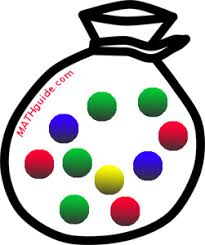
\includegraphics[width=1.4in]{marbles.jpg}
\end{figure}

Draw from replacement 37 times. What is the probability of getting 10 red, 17 green, 6 blue and 4 yellow? Compute explicitly to the nearest two significant digits.}\spc{7}

\hardsubproblem{[MA] If $\X \sim \multinomial{n}{\p}$, prove that its JMF sums to one, i.e. $\sum_{\x \in \support{\X}} p_{\X}(\x) = 1$.}\spc{7}

\hardsubproblem{[MA] If $\X \sim \multinomial{n}{\p}$, prove that any marginal distribution is binomial with $n$ and $p_j$ as parameters i.e. 

\beqn
p_{X_j}(x_j) = \binomial{n}{p_j}
\eeqn

We only assumed this in class because it makes sense conceptual given balls being sampled from an urn, but it was never explicitly proven.}\spc{9}

\extracreditsubproblem{[MA] If $\X \sim \multinomial{n}{\p}$, find the JMF of any subset of $X_1, \ldots, X_k$. Is it technically multinomial? This is not much harder than the previous problem if formulated carefully.}\spc{8}

\intermediatesubproblem{Explain in English why the following should be true. Remember how the sampling from the bag works.

\beqn
\B_1, \ldots, \B_n \iid \multinomial{1}{\p} \quad \text{then} \quad \X := \sum_{i=1}^n \B_i \sim \multinomial{n}{\p}
\eeqn}\spc{4}

\intermediatesubproblem{Find the answer by reasoning in English. No need to prove mathematically.

\beqn
\X_1, \ldots, \X_r \iid \multinomial{n}{\p} \quad \text{then} \quad \T := \sum_{i=1}^r \X_i \sim ~?
\eeqn}\spc{2}


\easysubproblem{If $\X \sim \multinomial{n}{\p}$, find $p_{\X_{-j}|X_{j}}(\x_{-j}, x_j)$ . This is marked easy since it's in the notes.}\spc{10}

\extracreditsubproblem{[MA] If $\X \sim \multinomial{n}{\p}$, find a proof for $\cov{X_i}{X_j} = -np_i p_j$ that is qualitatively different than the one we did in class.}\spc{12}

\intermediatesubproblem{If $\X \sim \multinomial{n}{\p}$ where $\dime{\X} = K$ and $\p = \oneover{K}\onevec_K$. What is the limit of  $\cov{X_i}{X_j}$ as $K$ gets large but $n$ is fixed. Why does this make sense?}\spc{5}

\easysubproblem{Correlation $\rho$ is a unitless measure bounded between $\bracks{-1, 1}$ and is a type of normalized covariance metric. It is defined for two r.v.'s as 

\beqn
\rho_{1,2} := \corr{X_1,\,X_2} := \frac{\sigma_{1,2}}{\sigma_1 \sigma_2} = \frac{\cov{X_1}{X_2}}{\sd{X_1} \sd{X_2}} = \frac{\cov{X_1}{X_2}}{\sqrt{\var{X_1} \var{X_2}}}
\eeqn

where $\sd{\cdot}$ denotes the standard deviation of a r.v., the square root of its variance. Find $\corr{X_i,\,X_j}$ for two arbitrary elements in the r.v. vector $\X \sim \multinomial{n}{\p}$. }\spc{3}



\easysubproblem{If $\c = \bracks{1 ~2 ~3 ~4}^\top$, compute the inner product $\c^\top \c$ and the outer product $\c \c^\top$.}\spc{10}

\end{enumerate}


\end{document}








\problem{These exercises give you practice with sums and indicator functions.}

\begin{enumerate}

\easysubproblem{Expand and simplify as much as you can: $\sum_{x \in \reals} \indic{x = 17}$.}\spc{0.5}

\easysubproblem{Expand and simplify as much as you can: $\sum_{x \in \reals} c \indic{x = 17}$ where $c \in \reals$ is a constant.}\spc{0.5}

\easysubproblem{Expand and simplify as much as you can: $\sum_{x \in \reals} \indic{x \in \braces{1, 2, 3}}$.}\spc{0.5}

\easysubproblem{Expand and simplify as much as you can: $\sum_{x \in \reals} x\indic{x \in \braces{1, 2, 3}}$.}\spc{0.5}
\easysubproblem{Expand and simplify as much as you can: $\sum_{x \in \naturals_0} x^{\indic{x \in \braces{1, 2, 3}}}$.}\spc{0.5}

\easysubproblem{Expand and simplify as much as you can: $\prod_{x \in \reals} \indic{x \in \braces{1, 2, 3}}$.}\spc{0.5}

\easysubproblem{Expand and simplify as much as you can: $\sum_{x \in \reals} \indic{x \in \braces{1, 2, 3}}\indic{x \in \braces{4, 5, 6}}$.}\spc{0.5}


\intermediatesubproblem{Expand and simplify as much as you can: $\sum_{x \in \reals} c \indic{x \in \braces{1, 2, \ldots, t}}$ where $c \in \reals$ is a constant and $t \in \naturals$ is a constant.}\spc{0.5}

\intermediatesubproblem{Expand and simplify as much as you can: $\sum_{x \in \reals} t \indic{x \in \braces{1, 2, \ldots, t}}$ where $c \in \reals$ is a constant and $t \in \naturals$ is a constant.}\spc{0.5}

\intermediatesubproblem{Expand and simplify as much as you can: $\sum_{x \in \reals} x \indic{x \in \braces{1, 2, \ldots, t}}$ where $c \in \reals$ is a constant and $t \in \naturals$ is a constant.}\spc{0.5}

\intermediatesubproblem{Expand and simplify as much as you can: $\sum_{x \in \reals} \oneover{x!} \indic{x \in \naturals}$.}\spc{0.5}

\intermediatesubproblem{Prove $\expe{\indic{X \in A}} = \prob{X \in A}$.}\spc{2}


\end{enumerate}

\problem{These exercises review convolutions.}


\begin{enumerate}

\easysubproblem{Is a JMF a type of PMF or PMF a type of JMF? Explain.}\spc{2}

\easysubproblem{Let $X_1, X_2 \iid \bernoulli{p}$. Find the PMF of the sum of $T = X_1 + X_2$ using the appropriate discrete convolution formula that would make the problem easiest.}\spc{4}

\easysubproblem{Let $X_1 \sim \bernoulli{p_1}$ independent of $X_2 \sim \bernoulli{p_2}$. Find the JMF of for $X_1, X_2$. Denote it using a 2 $\times$ 2 grid or the piecewise function notation.}\spc{6}

\easysubproblem{Use the JMF of for $X_1, X_2$ to find the PMF for $T = X_1 + X_2$. Denote it using the piecewise function notation.}\spc{3}

\intermediatesubproblem{Prove the PMF of $T = X_1 + X_2$ using the appropriate discrete convolution formula . Show that the function reduces to the piecewise function in (c) when substituting for the values of $t$. }\spc{6}


\hardsubproblem{Let 

\beqn
X_1 \sim \begin{cases}
3 \withprob 0.3 \\
6 \withprob 0.7
\end{cases} \quad \text{independent of} \quad
%
X_2 \sim \begin{cases}
4 \withprob 0.4 \\
8 \withprob 0.6
\end{cases} 
\eeqn

Find the PMF of $T = X_1 + X_2$ using a convolution. Denote it using the piecewise function notation.}\spc{8}


\hardsubproblem{Prove the PMF of a binomial inductively using convolutions on the sequence of r.v.'s $\Xoneton \iid \bernoulli{p}$. You will need to use Pascal's Triangle combinatorial identity we employed in class.}\spc{9}


\hardsubproblem{[MA] Prove the PMF of a negative binomial inductively using convolutions on the sequence of r.v.'s $\Xoneton \iid \geometric{p}$. You will need to use the \href{https://en.wikipedia.org/wiki/Hockey-stick_identity}{hockey stick identity}.}\spc{9}

\hardsubproblem{Let $X_1 \sim \binomial{n_1}{p}$ independent of $X_2 \sim \binomial{n_2}{p}$. Find the PMF of the sum of $T = X_1 + X_2$ using a convolution.}\spc{13}


\easysubproblem{Prove the PMF of $X \sim \poisson{\lambda}$ using the limit as $n \rightarrow \infty$ and let $p = \overn{\lambda}$.}\spc{9}


\hardsubproblem{Let $X_1 \sim \poisson{\lambda_1}$ independent of $X_2 \sim \poisson{\lambda_2}$. Find the PMF of the sum of $T = X_1 + X_2$ using a convolution.}\spc{8}



\end{enumerate}


\problem{These exercises introduce probabilities of conditional subsets of the supports of multiple r.v.'s.}


\begin{enumerate}

\hardsubproblem{Let $X \sim \geometric{p_x}$ independent of $Y \sim \geometric{p_y}$. Find $\prob{X > Y}$ using the method we did in class.}\spc{10}


\easysubproblem{[MA] Prove this a different way by finding $\prob{X = Y}$ and then using the law of total probability.}\spc{10}

\easysubproblem{[MA] As both $p_x$ and $p_y$ are reduced to zero, but $r = \frac{p_x}{p_y}$, what is the asymptotic probability you found in (a)?}\spc{10}

\hardsubproblem{Let $X \sim \poisson{\lambda}$ independent of $Y \sim \poisson{\lambda}$. Find an expression for $\prob{X > Y}$ \emph{as best as you are able to answer}. Part of this exercise is identifying where you cannot go any further.}\spc{9}


\end{enumerate}


\problem{These exercises will introduce the Multinomial distribution.}


\begin{enumerate}

\easysubproblem{If $\X \sim \multinomial{n}{\p}$ where $\dime{\X} = k$, what is the parameter space for both $n$ and $\p$?}\spc{2}

\easysubproblem{If $\X \sim \multinomial{n}{\p}$ where $\dime{\X} = k$, what is the $\support{\X}$?}\spc{2}

\easysubproblem{If $\X \sim \multinomial{n}{\p}$ where $\dime{\X} = k$, what is $\dime{\p}$?}\spc{-0.5}

\easysubproblem{If $\X \sim \multinomial{n}{\p}$ where $\dime{\X} = 2$, express $p_2$ as a function of $p_1$.}\spc{2}

\easysubproblem{If $\X \sim \multinomial{n}{\p}$ where $\dime{\X} = 2$, how are both $X_1$ and $X_2$ distributed?}\spc{1}

\easysubproblem{If $\X \sim \multinomial{n}{\p}$ and $n= 10$ and $\dime{\X} = 7$ as a column vector, give an example value of $\x$, a realization of the r.v. $\X$.}\spc{2}

\easysubproblem{If $\X \sim \multinomial{9}{\bracks{0.1~0.2~0.7}^\top}$, find $\prob{\X = \bracks{3~2~4}^\top}$ to the nearest two significant digits.}\spc{2}


%\intermediatesubproblem{If $\X \sim \multinomial{n}{\p}$ and $n= 10$ and $\p = \bracks{0.2, 0.8}^\top$, find $\muvec := \expe{\X}$.}\spc{2}


\hardsubproblem{[MA] If $\X_1 \sim \multinomial{n}{\p}$ and independently $\X_2 \sim \multinomial{n}{\p}$ where $\dime{\X_1} = \dime{\X_2} = k$. Find the JMF of $\T_2 = \X_1 + \X_2$ from the definition of convolution. This looks harder than it is! First, use the definition of convolution and factor out the terms that are not a function of $x_1, \ldots, x_K$. Finally, use Theorem 1 in \href{http://www.lrecits.usthb.dz/1.3.pdf}{this paper} for the summation.}\spc{9}

\end{enumerate}


\end{document}

